\section{Total internal reflection and frustrated TIR}

The third example probes the same single-interface machinery beyond the
critical angle and then promotes the geometry to a three-layer stack in
order to resolve the evanescent tunnelling known as frustrated total
internal reflection (FTIR). The incident medium is glass ($n_1 = 1.50$)
and the transmitted medium is air ($n_2 = 1.00$) at
$\lambda = \SI{550}{\nano\metre}$, so the critical angle is
$\theta_c = \arcsin(n_2/n_1) = \SI{41.81}{\degree}$. Above $\theta_c$ no
real transmission angle exists; the normal component of the wavevector in
air becomes imaginary, and unitarity demands
\begin{equation}
  R(\theta > \theta_c) = 1. \label{eq:tir-R}
\end{equation}
Panel (a) of Fig.~\ref{fig:tir} plots $|1 - R|$ for $s$- and
$p$-polarisation on a logarithmic scale across the forbidden window
$\theta_c < \theta < \SI{89}{\degree}$. Panel (b) compares the unwrapped
phase of $r_s$ to the textbook closed form
\begin{equation}
  \tan\!\left(\frac{\delta_s}{2}\right) = \frac{\sqrt{\sin^{2}\theta - (n_2/n_1)^{2}}}{\cos\theta}. \label{eq:tir-phase}
\end{equation}

Panel (c) inserts a finite air gap of variable thickness $d$ between two
glass half-spaces, so the stack becomes glass\,/\,air\,/\,glass with a
single finite layer. Above $\theta_c$ the wave in the gap is evanescent,
with imaginary out-of-plane wavenumber $q_2 = \ii\kappa$ and
$\kappa = k_0\sqrt{n_1^{2}\sin^{2}\theta - n_2^{2}}$. The three-layer
Airy transmittance then reads
\begin{equation}
  t = \frac{t_{12}\,t_{21}\,e^{\ii q_2 d}}{1 - r_{12}^{2}\,e^{2\ii q_2 d}},\qquad T = |t|^{2}, \label{eq:ftir-T}
\end{equation}
which is evaluated at $\theta = \SI{60}{\degree}$ for gap thicknesses from
\SI{10}{\nano\metre} to \SI{600}{\nano\metre} and overlaid on the TMM
result.

\begin{center}
\begin{tikzpicture}
  \fill[blue!6]  (0, 0) rectangle (5, 1.6);
  \fill[yellow!15] (0,-0.6) rectangle (5, 0);
  \fill[blue!6]  (0,-1.8) rectangle (5,-0.6);
  \draw[thick] (0,0) -- (5,0);
  \draw[thick] (0,-0.6) -- (5,-0.6);
  \node[lbl, anchor=east] at (4.9, 1.2) {glass $n_1$};
  \node[lbl, anchor=east] at (4.9,-0.3) {air $n_2$, $d$};
  \node[lbl, anchor=east] at (4.9,-1.3) {glass $n_1$};
  \raysketch{1.6}{55}{t}
\end{tikzpicture}
\end{center}

\begin{figure}[!htbp]
  \centering
  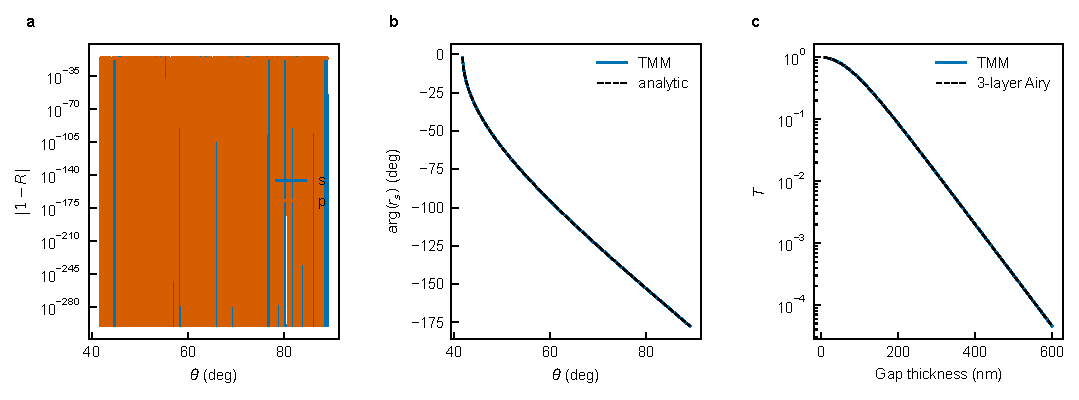
\includegraphics[width=\textwidth]{03_tir_and_ftir.pdf}
  \caption{(a) $|1-R|$ above $\theta_c$ for $s$ and $p$ polarisation. (b) Phase of $r_s$ versus the closed form~\eqref{eq:tir-phase}. (c) Frustrated-TIR transmittance $T(d)$ at \SI{60}{\degree} against the exact three-layer Airy expression~\eqref{eq:ftir-T}.}
  \label{fig:tir}
\end{figure}

Above $\theta_c$ the TMM returns unit reflectance to
$|1-R| \approx \num{9e-16}$ for both polarisations, and the reflection
phase tracks~\eqref{eq:tir-phase} to the same tolerance. The FTIR curve
agrees with the closed-form Airy transmittance at
$\max|\Delta T| \approx \num{7e-16}$ down to sub-nanometre gaps. The
transmittance follows the pure exponential $e^{-2\kappa d}$ for
$d \gg \kappa^{-1}$, but deviates visibly from it below
$d \lesssim \SI{100}{\nano\metre}$; in that near-gap regime the Fresnel
prefactors of~\eqref{eq:ftir-T} matter, and the TMM tracks those
corrections exactly.


